\section{NodeJS}
\label{sec:chapter_tecnologie_abilitanti_nodejs}

Node.js è un framework open-source, multi-piattaforma che permette lo sviluppo di applicazioni web lato server scritte in JavaScript ed eseguibili su Linux, Microsoft Windows ed OS X.
La piattaforma è costruita sull’ engine Javascript runtime V8 di Google, utilizzato anche da Chrome/Chromium.
\\
Node.js nasce con l’ obiettivo di facilitare la realizzazione di applicazioni web lato server, contenendo a tal proposito librerie integrate per la creazione di web-server altamente scalabili.
Esso non sfrutta il classico modello basato su processi o thread concorrenti ma prevede una architettura basata su singolo thread ed una API di I/O non bloccante, fondamentale per la creazione di applicazioni web real-time altamente produttive e scalabili. \cite{node2}
\\
Nello specifico lo sviluppatore utilizza un modello asincrono di programmazione basato su eventi in cui vengono eseguite azioni solo al verificarsi di uno specifico evento. 
Quando ad esempio viene richiesto un valore ad un server remoto, l’istruzione che ha effettuato la richiesta non blocca l’esecuzione ma viene saltata.
\\
In questo modo l’esecuzione è in grado di proseguire con le istruzioni successive senza dover attendere il valore richiesto.
\\
La funzione di callback viene eseguita solamente quando è completata la chiamata remota ed il controllo dell’ esecuzione è tornato all’istruzione sospesa.
Questo metodo garantisce un’ ottimizzazione delle performance quando si lavora su web. 
I tempi di attesa tra una richiesta HTTP e l’ altra risulterebbero, infatti, troppo lunghi rispetto ai tempi di lavoro del processore e quindi attendere una risposta rallenterebbe troppo il sistema.
\\
Ogni funzione in Node.js è asincrona, quindi le istruzioni che normalmente bloccherebbero il thread vengono invece eseguite in background. \cite{node1}
\\
\begin{figure}[htb]
 \centering
 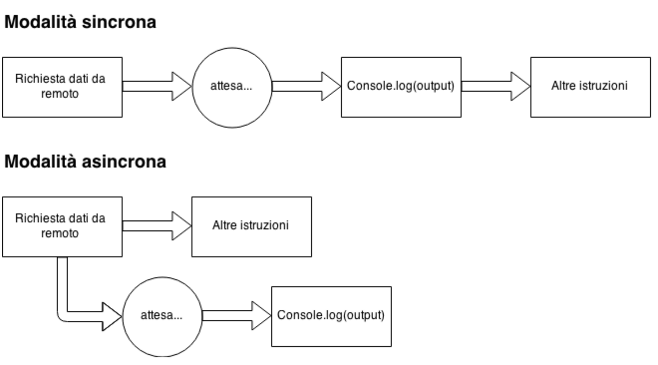
\includegraphics[width=0.9\linewidth]{images/chapter_tecnologie_abilitanti/tecnologie_abilitanti_node_mod.png}\hfill
 \caption[NodeJS: modalità sincrona e asincrona]{Differenza tra modalità sincrona e asincrona}
 \label{fig:tecnologie_abilitanti_node_mod}
\end{figure}
\\
Ad esempio per leggere un file in maniera asincrona bisogna specificare una funzione di callback da eseguire una volta che l’ operazione di lettura è stata completata.
La callback è una funzione che viene chiamata solo dopo che un dato task è stato completato.
Un esempio di callback è il seguente :
\begin{lstlisting}[language=javascript]
var callback = function(err, contents) {
	console.log(contents);
}
fs.readFile('etc/hosts', callback);
console.log('Fai qualcos\'altro...');
\end{lstlisting}
Il codice è non-bloccante in quanto la funzione che esegue la lettura inizia a leggere il file e ritorna immediatamente il controllo all’ambiente di esecuzione, permettendo l’esecuzione delle istruzioni successive( stampa a video di una stringa nell’esempio). 
La callback viene invocata solamente quanto il file è stato letto.
\\
Quindi le callback rappresentano un approccio comodo e molto utilizzato soprattutto nelle interazioni con il server; tuttavia il loro utilizzo in situazioni complesse può presentare problemi.
\\
Quando ad esempio viene sottomessa ad un server una richiesta per l’elenco dei post e delle foto pubblicati sul blog di un utente, vengono effettuate tre chiamate al metodo \texttt{get()}. 
Ciascuna \texttt{get()} ha la relativa funzione di callback (passata come terzo argomento), che viene eseguita quando il server restituisce il risultato richiesto.
\begin{lstlisting}
$.get("/users", {id: "12345"},
 function(user) {
  $.get("/blogs", {id: user.blogId},
   function(blog) {
   	displayPostList(blog.posts);
   });
  $.get("/photos", {id: user.albumId},
   function(album) {
   	displayPhotoList(album.photos);
   }
  );	
 }
);
\end{lstlisting}
La prima callback viene invocata quando la prima get restituisce la rappresentazione json dell’ utente richiesto. Le altre 2 get sono annidate dentro la prima callback in quanto dipendenti dall’esito della prima chiamata.
\\ 
Visto che la visualizzazione dei post e delle foto è asincrona, non necessariamente quest’ultime verranno visualizzate dopo i post. Quindi per vincolare l’ordine di visualizzazione o per effettuare ulteriori elaborazioni su entrambi gli insiemi di risultati prima di visualizzarli (come mostrare solo le foto relative ai post), bisogna trovare un modo per sincronizzare le callback; cosa tutt’altro che semplice.
\\
Da questo esempio quindi è possibile notare i principali difetti derivanti da un uso intensivo delle callback:
\begin{itemize}
\item Scarsa leggibilità del codice, che tende facilmente a svilupparsi verso destra a causa dei molteplici annidamenti delle callback.
\item Difficoltà di composizione delle callback e di sincronizzazione del flusso di elaborazione.
\item Difficoltà nella gestione degli errori e nel debug, soprattutto in presenza di callback anonime. Non è possibile infatti gestire l’eccezione all’interno della funzione chiamante la callback.
\end{itemize}
Il problema principale è che dall’ esecuzione di chiamate asincrone, diversamente da quelle sincrone, non si ottiene un valore di ritorno o una eccezione. Non è possibile quindi la composizione di funzioni e la gestione di eventuali eccezioni.
Per questo motivo l’api di node, che prima faceva solamente uso delle callback, permette ora anche l’utilizzo delle promesse. \cite{node4}
\\
Le promesse, o promise, sono oggetti che rappresentano il risultato di una chiamata di funzione asincrona. L’ oggetto, nel dettaglio, rappresenta la promessa che un risultato verrà fornito non appena disponibile.
Il vantaggio principale nell’utilizzo delle promesse rispetto alle callback consiste nel rendere il codice più leggibile in quanto più simile al flusso di esecuzione sincrono.
La componente principale dell’oggetto promessa è il suo metodo then. 
Il metodo then viene invocato una volta ottenuto il risultato dell’ operazione asincrona e prende come argomento due callback opzionali, una eseguita quando l’operazione è andata a buon fine, l’altra in caso di errore.
\begin{lstlisting}[language=javascript]
var promise = doSomethingAsync();
promise.then(onFulfilled, onRejected);
\end{lstlisting}
Il conclusione quindi il fatto che Node.js operi su thread singolo ed utilizzi chiamate I/O non bloccanti, piuttosto che usare thread concorrenti, permette il supporto di decine di migliaia di connessioni senza pagare il costo dovuto al cambiamento di contesto; risultando quindi ideale per applicazioni real-time altamente concorrenti, applicazioni I/O bound, applicazioni data streaming. \cite{node3}
\\
Operare con un singolo thread però non consente la scalatura orizzontale; non comporta quindi benefici in termini di prestazioni all’ aumentare numero di processori fisici. 
Per questo motivo non è consigliabile utilizzare Node.js per applicazioni che fanno utilizzo intensivo della CPU.
Nel presente lavoro di tesi Node.js ha permesso la creazione di un server in grado di accettare richieste concorrenti da parte dei client, i dettagli verrano esaminati nei capitoli successivi.

